\newcommand{\gripperFloor}[3]
{
    \draw [ultra thick] (#1,#2) -- (#1 + 0.6, #2);
    \draw [ultra thick] (#1 + 0.8, #2) -- (#1 + 1.4,#2);
    \node [draw,minimum size=0.65cm] at (#1 + 0.7, #2 - 0.75) {$s_#3$};

}

\newcommand{\gripperHand}[2]
{
    \draw [ultra thick] (#1 + 0.3,#2) -- (#1 + 0.3, #2 + 0.4);
    \draw [ultra thick] (#1, #2 - 0.4) --(#1,#2) -- (#1 + 0.6,#2) -- (#1 + 0.6, #2 - 0.4);
}

\newcommand{\gripperBall}[2]
{
    \draw [ultra thick] (#1,#2) circle [radius=0.225];
}

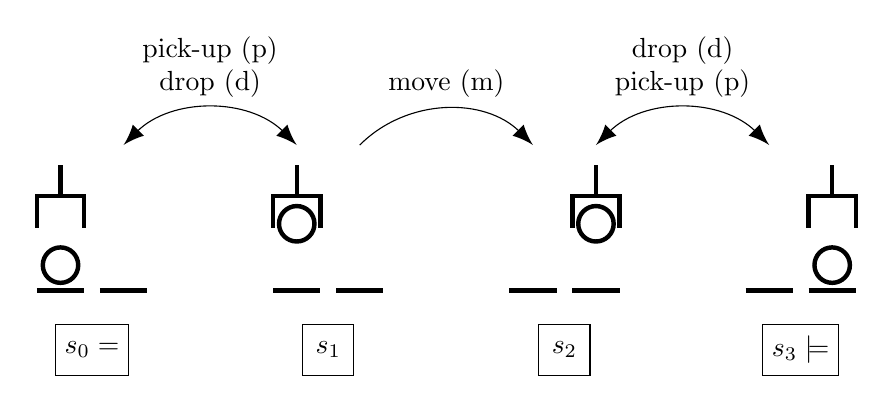
\begin{tikzpicture}[]
    \gripperFloor{0}{0}{0 = \init}
    \gripperBall{0.3}{0.325}
    \gripperHand{0.0}{1.2}

    \gripperFloor{3}{0}{1}
    \gripperBall{3.3}{0.85}
    \gripperHand{3}{1.2}

    \gripperFloor{6}{0}{2}
    \gripperBall{7.1}{0.85}
    \gripperHand{6.8}{1.2}

    \gripperFloor{9}{0}{3 \models \goal}
    \gripperBall{10.1}{0.325}
    \gripperHand{9.8}{1.2}

    \draw[>=latex, <->] (1.1,1.85) to[ultra thick, bend left=45] node [above, align=center] {pick-up (p) \\ drop (d)} (3.3,1.85);
    \draw[>=latex, ->] (4.1,1.85) to[ultra thick, bend left=45] node [above, align=center] {move (m)} (6.3,1.85);
    \draw[>=latex, <->] (7.1,1.85) to[ultra thick, bend left=45] node [above, align=center] {drop (d) \\ pick-up (p)} (9.3,1.85);

    \node at (0,-1.1) {};

    %\draw [ultra thick, dashed] (0,-1) -- (7, -1);
\end{tikzpicture}
